\documentclass[]{exam}
\usepackage{lmodern}
\usepackage{amssymb,amsmath}
\usepackage{ifxetex,ifluatex}
\usepackage{fixltx2e} % provides \textsubscript
\ifnum 0\ifxetex 1\fi\ifluatex 1\fi=0 % if pdftex
  \usepackage[T1]{fontenc}
  \usepackage[utf8]{inputenc}
\else % if luatex or xelatex
  \ifxetex
    \usepackage{mathspec}
    \makeatletter % undo the wrong changes made by mathspec
    \let\RequirePackage\original@RequirePackage
    \let\usepackage\RequirePackage
    \makeatother
  \else
    \usepackage{fontspec}
  \fi
  \defaultfontfeatures{Ligatures=TeX,Scale=MatchLowercase}
\fi
% use upquote if available, for straight quotes in verbatim environments
\IfFileExists{upquote.sty}{\usepackage{upquote}}{}
% use microtype if available
\IfFileExists{microtype.sty}{%
\usepackage{microtype}
\UseMicrotypeSet[protrusion]{basicmath} % disable protrusion for tt fonts
}{}
\usepackage{hyperref}
\hypersetup{unicode=true,
            pdftitle={Homework 1},
            pdfborder={0 0 0},
            breaklinks=true}
\urlstyle{same}  % don't use monospace font for urls
\IfFileExists{parskip.sty}{%
\usepackage{parskip}
}{% else
\setlength{\parindent}{0pt}
\setlength{\parskip}{6pt plus 2pt minus 1pt}
}
\setlength{\emergencystretch}{3em}  % prevent overfull lines
\providecommand{\tightlist}{%
  \setlength{\itemsep}{0pt}\setlength{\parskip}{0pt}}
\setcounter{secnumdepth}{0}
% Redefines (sub)paragraphs to behave more like sections
\ifx\paragraph\undefined\else
\let\oldparagraph\paragraph
\renewcommand{\paragraph}[1]{\oldparagraph{#1}\mbox{}}
\fi
\ifx\subparagraph\undefined\else
\let\oldsubparagraph\subparagraph
\renewcommand{\subparagraph}[1]{\oldsubparagraph{#1}\mbox{}}
\fi

\title{Homework 1}
\date{September 14, 2025}

\usepackage[margin=.75in]{geometry}
\RequirePackage{amsmath}
\usepackage{amssymb}
\usepackage{textcase}
\usepackage{soul}
\usepackage{indentfirst}

\newcommand{\eps}{\varepsilon}
\newcommand{\kron}{\otimes}
\DeclareMathOperator{\diag}{diag}
\DeclareMathOperator{\trace}{trace}
\DeclareMathOperator{\tvec}{vec}
\DeclareMathOperator{\rank}{rank}
\DeclareMathOperator{\tspan}{span}
\DeclareMathOperator*{\minimize}{minimize}
\DeclareMathOperator*{\maximize}{maximize}
\DeclareMathOperator{\subjectto}{subject\ to}

\newcommand{\mat}[1]{\boldsymbol{#1}}
\renewcommand{\vec}[1]{\boldsymbol{\mathrm{#1}}}
\newcommand{\vecalt}[1]{\boldsymbol{#1}}

\newcommand{\conj}[1]{\overline{#1}}

\newcommand{\normof}[1]{\|#1\|}
\newcommand{\onormof}[2]{\|#1\|_{#2}}

\newcommand{\MIN}[2]{\begin{array}{ll} \displaystyle \minimize_{#1} & {#2} \end{array}}
\newcommand{\MINone}[3]{\begin{array}{ll} \displaystyle \minimize_{#1} & {#2} \\ \subjectto & {#3} \end{array}}
\newcommand{\OPTone}{\MINone}
\newcommand{\MINthree}[5]{\begin{array}{ll} \displaystyle \minimize_{#1} & {#2} \\ \subjectto & {#3} \\ & {#4} \\ & {#5} \end{array}}

\newcommand{\MAX}[2]{\begin{array}{ll} \displaystyle \maximize_{#1} & {#2} \end{array}}
\newcommand{\MAXone}[3]{\begin{array}{ll} \displaystyle \maximize_{#1} & {#2} \\ \subjectto & {#3} \end{array}}


\newcommand{\itr}[2]{#1^{(#2)}}
\newcommand{\itn}[1]{^{(#1)}}

\newcommand{\prob}{\mathbb{P}}
\newcommand{\probof}[1]{\prob\left\{ #1 \right\}}

\newcommand{\pmat}[1]{\begin{pmatrix} #1 \end{pmatrix}}
\newcommand{\bmat}[1]{\begin{bmatrix} #1 \end{bmatrix}}
\newcommand{\spmat}[1]{\left(\begin{smallmatrix} #1 \end{smallmatrix}\right)}
\newcommand{\sbmat}[1]{\left[\begin{smallmatrix} #1 \end{smallmatrix}\right]}

\newcommand{\RR}{\mathbb{R}}
\newcommand{\CC}{\mathbb{C}}

\providecommand{\eye}{\mat{I}}
\providecommand{\mA}{\ensuremath{\mat{A}}}
\providecommand{\mB}{\ensuremath{\mat{B}}}
\providecommand{\mC}{\ensuremath{\mat{C}}}
\providecommand{\mD}{\ensuremath{\mat{D}}}
\providecommand{\mE}{\ensuremath{\mat{E}}}
\providecommand{\mF}{\ensuremath{\mat{F}}}
\providecommand{\mG}{\ensuremath{\mat{G}}}
\providecommand{\mH}{\ensuremath{\mat{H}}}
\providecommand{\mI}{\ensuremath{\mat{I}}}
\providecommand{\mJ}{\ensuremath{\mat{J}}}
\providecommand{\mK}{\ensuremath{\mat{K}}}
\providecommand{\mL}{\ensuremath{\mat{L}}}
\providecommand{\mM}{\ensuremath{\mat{M}}}
\providecommand{\mN}{\ensuremath{\mat{N}}}
\providecommand{\mO}{\ensuremath{\mat{O}}}
\providecommand{\mP}{\ensuremath{\mat{P}}}
\providecommand{\mQ}{\ensuremath{\mat{Q}}}
\providecommand{\mR}{\ensuremath{\mat{R}}}
\providecommand{\mS}{\ensuremath{\mat{S}}}
\providecommand{\mT}{\ensuremath{\mat{T}}}
\providecommand{\mU}{\ensuremath{\mat{U}}}
\providecommand{\mV}{\ensuremath{\mat{V}}}
\providecommand{\mW}{\ensuremath{\mat{W}}}
\providecommand{\mX}{\ensuremath{\mat{X}}}
\providecommand{\mY}{\ensuremath{\mat{Y}}}
\providecommand{\mZ}{\ensuremath{\mat{Z}}}
\providecommand{\mLambda}{\ensuremath{\mat{\Lambda}}}
\providecommand{\mSigma}{\ensuremath{\mat{\Sigma}}}
\providecommand{\mPbar}{\bar{\mP}}

\providecommand{\ones}{\vec{e}}
\providecommand{\va}{\ensuremath{\vec{a}}}
\providecommand{\vb}{\ensuremath{\vec{b}}}
\providecommand{\vc}{\ensuremath{\vec{c}}}
\providecommand{\vd}{\ensuremath{\vec{d}}}
\providecommand{\ve}{\ensuremath{\vec{e}}}
\providecommand{\vf}{\ensuremath{\vec{f}}}
\providecommand{\vg}{\ensuremath{\vec{g}}}
\providecommand{\vh}{\ensuremath{\vec{h}}}
\providecommand{\vi}{\ensuremath{\vec{i}}}
\providecommand{\vj}{\ensuremath{\vec{j}}}
\providecommand{\vk}{\ensuremath{\vec{k}}}
\providecommand{\vl}{\ensuremath{\vec{l}}}
\providecommand{\vm}{\ensuremath{\vec{m}}}
\providecommand{\vn}{\ensuremath{\vec{n}}}
\providecommand{\vo}{\ensuremath{\vec{o}}}
\providecommand{\vp}{\ensuremath{\vec{p}}}
\providecommand{\vq}{\ensuremath{\vec{q}}}
\providecommand{\vr}{\ensuremath{\vec{r}}}
\providecommand{\vs}{\ensuremath{\vec{s}}}
\providecommand{\vt}{\ensuremath{\vec{t}}}
\providecommand{\vu}{\ensuremath{\vec{u}}}
\providecommand{\vv}{\ensuremath{\vec{v}}}
\providecommand{\vw}{\ensuremath{\vec{w}}}
\providecommand{\vx}{\ensuremath{\vec{x}}}
\providecommand{\vy}{\ensuremath{\vec{y}}}
\providecommand{\vz}{\ensuremath{\vec{z}}}
\providecommand{\vpi}{\ensuremath{\vecalt{\pi}}}

\providecommand{\vlambda}{\ensuremath{\vecalt{\lambda}}}


\sodef\allcapsspacing{\upshape}{0.15em}{0.65em}{0.6em}%

\makeatletter
\def\maketitle{%
\par
\hrule height 0.75pt\vspace{1ex}
\par\noindent
\begin{minipage}{0.5\textwidth}
\scshape
purdue university $\cdot$ cs 51500 \\
matrix computations
\end{minipage}
\begin{minipage}{0.5\textwidth}
\raggedleft
\MakeTextUppercase{\allcapsspacing{\@title}}\\[0.2ex]
\textit{\@author}\\[0.2ex]
\textit{\@date}
\end{minipage}
\par\vspace{1ex}
\hrule height 1pt
\vspace{2ex}
\par
}
\makeatother

\author{Jinen Setpal}
\title{Lecture Notes}
% auto generate a title
% \AtBeginDocument{\maketitle}

\title{Homework 1 Submission}

% Question header formatting
\qformat{\hfill \textbf{Problem \thequestion} \hfill}

\DeclareMathOperator{\Tr}{Tr}
\DeclareMathOperator{\Cov}{Cov}
\DeclareMathOperator{\Concat}{Concat}
\DeclareMathOperator*{\argsup}{arg\,sup}
\DeclareMathOperator*{\arginf}{arg\,inf}
\DeclareMathOperator*{\argmax}{arg\,max}
\DeclareMathOperator*{\argmin}{arg\,min}
\DeclareMathOperator*{\indep}{\perp \!\!\! \perp}
\setcounter{MaxMatrixCols}{20}

\newcommand{\divider}{\line(1,0){\textwidth}}

\allowdisplaybreaks

% Package for enumerated lists using letters
\usepackage{enumitem}

% Algorithms
\usepackage{algpseudocode}
\usepackage{algorithm}
\usepackage{nicefrac}
\usepackage{graphicx}
\usepackage{fancyvrb,fvextra}
\usepackage[usenames,dvipsnames]{xcolor}
\usepackage{listings}
\usepackage{hyperref}

%%
%% Julia definition (c) 2014 Jubobs
%%
\lstdefinelanguage{Julia}%
  {morekeywords={abstract,break,case,catch,const,continue,do,else,elseif,%
      end,export,false,for,function,immutable,import,importall,if,in,%
      macro,module,otherwise,quote,return,switch,true,try,type,typealias,%
      using,while},%
   sensitive=true,%
   alsoother={$},%
   morecomment=[l]\#,%
   morecomment=[n]{\#=}{=\#},%
   morestring=[s]{"}{"},%
   morestring=[m]{'}{'},%
}[keywords,comments,strings]%

\lstset{%
    language         = Julia,
    basicstyle       = \ttfamily,
    keywordstyle     = \bfseries\color{blue},
    stringstyle      = \color{magenta},
    commentstyle     = \color{ForestGreen},
	breaklines=true,
    showstringspaces = false,
}

\begin{document}
\maketitle

\hypertarget{problem-0-homework-checklist}{%
\subsection{Checklist}\label{problem-0-homework-checklist}}


\begin{enumerate}
	\item Cross-checked independent work with Kunal Kapur.
	\item No use of AI tools.
	\item Code is included!
\end{enumerate}

\begin{questions}

\question
\hfill

\begin{enumerate}[label=\arabic*.]
	\item Each element across the diagonal scales the corresponding row vector proportionally. Thus, we have:
		$$\bmat{2 & 0 & 0 \\ 0 & 1/2 & 0 \\ 0 & 0 & -1} \bmat{ 1 & 2 & 3 \\ 6 & 4 & 2 \\ -2 & -2 & -2 } = \bmat{ 2 & 4 & 6 \\ 3 & 2 & 1 \\ 2 & 2 & 2 }$$
	\item Setting the diagonal matrix as the transformation makes it easier to compute. By transposition, we have: $\mA \mB = (\mB^T \mA^T)^T$
		\begin{align*}
			\bmat{ 1 & 2 & 3 \\ 6 & 4 & 2 \\ -2 & -2 & -2 } \bmat{2 & 0 & 0 \\ 0 & 1/2 & 0 \\ 0 & 0 & -1} &=
			\left( \bmat{2 & 0 & 0 \\ 0 & 1/2 & 0 \\ 0 & 0 & -1} \bmat{ 1 & 6 & -2 \\ 2 & 4 & -2 \\ 3 & 2 & -2 } \right)^T \\
			\intertext{We can now apply the same diagonal scaling as before:}
			 &= \left( \bmat{ 2 & 12 & -4 \\ 1 & 2 & -1 \\ -3 & -2 & 2 } \right)^T \\
			 \bmat{ 1 & 2 & 3 \\ 6 & 4 & 2 \\ -2 & -2 & -2 } \bmat{2 & 0 & 0 \\ 0 & 1/2 & 0 \\ 0 & 0 & -1} &= \bmat{ 2 & 1 & -3 \\ 12 & 2 & -2 \\ -4 & -1 & 2 }
		\end{align*}
	\item Using the result from the previous questions, we can merge the two right-most matrices, and then apply diagonal scaling.
		\begin{align*}
			\bmat{1/2 & 0 & 0 \\ 0 & 2 & 0 \\ 0 & 0 & -1} \bmat{ 1 & 2 & 3 \\ 6 & 4 & 2 \\ -2 & -2 & -2 } \bmat{2 & 0 & 0 \\ 0 & 1/2 & 0 \\ 0 & 0 & -1} &= \bmat{1/2 & 0 & 0 \\ 0 & 2 & 0 \\ 0 & 0 & -1} \bmat{ 2 & 1 & -3 \\ 12 & 2 & -2 \\ -4 & -1 & 2 } = \bmat{ 1 & .5 & -1.5 \\ 24 & 4 & -4 \\ 4 & 1 & -2 }
		\end{align*}
	\item Applying diagonal scaling on the left transforms the rows of the right matrix, whereas applying diagonal scaling on the right transforms the columns of the left matrix. In either case, the scaling applied corresponds to the diagonal element of the row / column vector respectively.
	\item We have $\vx, \vy \in \mathbb{R}^{1000 \times 1}$.
		\begin{align*}
			\vx^T \vy = \bmat{1 & 1 & \cdots & 1} \bmat{1 \\ 2 \\ \cdots \\ 1000} = \langle \vx, \vy \rangle = \sum^{1000}_{i=1} i = \frac{n (n + 1)}{2} = \frac{1001 \cdot 1000}{2} = 500500
		\end{align*}
	\item Let $\ve$ specifically represent the {\it column} vector. We are given $\mA \in \mathbb{R}^{m \times n}$.

		We can select the $r^{th}$ row by left multiplication: $\ve_r^T \mA$, and select the $c^{th}$ column by right multiplication: $\mA \ve_c$.
	\item We have $\vx = \bmat{-5 & 4 & 2}^T$ and $\ve_i \in \mathbb{R}^{3 \times 1}$. Assuming indexing starts with 1. Then,
		$$ \ve_2 \vx^T = \bmat{0 \\ 1 \\ 0} \bmat{-5 & 4 & 2} = \bmat{0 & 0 & 0 \\ -5 & 4 & 2 \\ 0 & 0 & 0 } $$
		and,
		$$ \vx \ve_1^T = \bmat{-5 \\ 4 \\ 2} \bmat{1 & 0 & 0} = \bmat{-5 & 0 & 0 \\ 4 & 0 & 0 \\ 2 & 0 & 0} $$
	\item Applying the column-selector idea, each of these operations are simply selecting columns. Thus, we have $\mA \ve_1 = \bmat{2 & 0 & 0}^T,~\mA \ve_2 = \bmat{0 & 1/2 & 0}^T,~\mA \ve_3 = \bmat{0 & 0 & -1}^T$
\end{enumerate}

\newpage
\question
\hfill

\begin{enumerate}[label=\arabic*.]
	\item The answer to this is highly dependent on the assumptions I make. Consider, \\
		\textbf{Scenario 1}: OpenAI has competent engineers. In this case:
		\begin{enumerate}[label=\alph*.]
			\item Their web crawler finds a database containing everyone's personal data, including the social security number. It is then formatted into a paragraph form where the personal data is preceded by the SSN.
			\item GPT-5 is trained on next-token prediction.
			\item Each SSN gets it's own encoding (as opposed to, e.g., each letter getting it's own embedding and then being concatenated to form the final SSN embedding) or each part (first three, next two, and last four digits) get their own embeddings which are then concatenated.
		\end{enumerate}
		\textbf{Consequence:} In this case, I'd argue the embeddings do constitute a matrix. A sufficiently well-trained GPT-5 should learn the correlation of SSNs with personal data, especially givenhistorically, the first three digits denote area (e.g., XXX-YY-ZZZZ was born in Austin, Texas). These could be embedded as specific columns within the embedding, or even as an unprivileged basis. Either way, it makes sense to perform linear transformations on this table, hence it's a matrix. \\

		\textbf{Scenario 2}: OpenAI has less competent engineers. In this case:
		\begin{enumerate}[label=\alph*.]
			\item They synthetically generate all SSNs, but don't have any associated data about the individual. This is then randomly sampled and spliced together using spaces into paragraph form for each batch.
			\item GPT-5 is trained on next-token prediction.
			\item Each character gets it's own encoding.
		\end{enumerate}
		\textbf{Consequence:} In this case, I'd argue the embeddings do not constitute a matrix. During training, the preceding data is entirely disconnected from and offers no insight into the next token. Further, each character is oversubscribed; repeated characters mean repeated encodings, making it harder still to obtain a meaningful result. The model cannot be well-trained and the embeddings are meaningless. The learned embeddings are a table of disconnected numbers. Performing linear transformations on this would lend no insight, hence this is not a matrix.
	\item Although I don't identify any structure (e.g., Hankel / Toeplitz), I do think this is a matrix. Audio is processed per second (assuming 44.1kHz) with each element representing the amplitude of the wave. As an example, we can compute the similar chunks of audio by computing the inner product of $\mA$.
	\item Each of the columns represent factors that are relevant to admission. Consider $\vx = \bmat{1 & 1 & 0 & 1 & 1 & 1}^T$. If $\mA$ is the described matrix, $\mA \vx$ is a very rudimentary way to score each applicant. We can then rank applicants by score and evaluate if it correlates strongly with their admission into Purdue's CS program. It makes sense to perform linear transformations on this data; therefore, this is an example of a matrix.
	\item For $N$ SSNs, we have $\mA \in \mathbb{R}^{N \times 3072}$. Thus $\mA^T \mA \in \mathbb{R}^{3072 \times 3072}$ renders the correlation between each of the embeddings. If we assume that GPT-5 embeddings are a matrix (in that they are meaningful), this is valuable as high similarity scores would denote correlated features, while low scores denote anti-correlated features. Both are useless and can be safely discarded (or a smaller embedding may be trained). If $\mA^T \mA \approx \mI$, we may conjecture that the embeddings are saturated.
	\item Similarity across for $N$ seconds of audio $A \in \mathbb{R}^{44100 \times N}$ results in comparing each second of audio to the other. Overlaps between segments will result in amplified scores, while anti-waves cancel one another out. We studied applications of linear algebra to noise cancelling as well; so I'd say this is safely a matrix too.
	\item For $N$ applicants, we have $\mA \in \mathbb{R}^{N \times 6}$. Thus $\mA^T \mA \in \mathbb{R}^{N \times N}$ denotes the correlation between factors; for the same reason as part 4, $\mA^T \mA$ is a matrix.
\end{enumerate}

\newpage
\question
\hfill

\begin{enumerate}[label=\arabic*.]
	\item Let $\mA = \bmat{a_{11} & & \\ & \ddots \\ & & a_{dd}},~\mB = \bmat{b_{11} & & \\ & \ddots \\ & & b_{dd}}$. We have the product rule:
		$$
		\mC = \mA \mB \qquad \text{where} \qquad \mC_{ij} = \sum^{d}_{k=1} \mA_{ik} \mB_{kj}
		$$
		It suffices to show that:
		$$
		\mA_{ij} = \mB_{ij} = 0 \implies
		\mC_{ij} = 0 \qquad \forall i \neq j
		$$
		Let $[d] = \{1, 2, \ldots, d\}$. We have that, for $i \neq j$,
		\begin{align*}
			\mC_{ij} &= \sum^{d}_{k=1} \mA_{ik} \mB_{kj} \\
			&= (\mA_{ii} \mB_{ij} + \mA_{ij} \mB_{jj}) + \sum_{k \in [d] \setminus \{i, j\}} \mA_{ik} \mB_{kj} \\
			&= (\mA_{ii} \cdot 0 + 0 \cdot \mB_{jj}) + \sum_{k \in [d] \setminus \{i, j\}} 0 = 0 
		\end{align*}
		Thus $\mC_{ij} = 0~\forall i \neq j$, and the resultant matrix $\mC$ is also diagonal.
	\item Let $\mA = \bmat{a_{1} & a_2 & \cdots & a_n \\ a_2 & a_3 & \cdots & a_{1} \\ \vdots & \vdots & & \vdots \\ a_n & a_1 & \cdots & a_{n-1}},~\mB = \bmat{b_{1} & b_2 & \cdots & b_n \\ b_2 & b_3 & \cdots & b_{1} \\ \vdots & \vdots & & \vdots \\ b_n & b_1 & \cdots & b_{n-1}}$

		Circulant matrices are those s.t:
		$$
		\mC_{ij} = \mC_{i + 1, j - 1}
		\qquad \text{where} \qquad
		\mC_{i,0} = \mC_{in},~\mC_{n+1,j} = \mC_{1,j}
		$$
		It suffices to show that:
		$$
		\mA_{ij} = \mA_{i + 1, j - 1},~
		\mB_{ij} = \mB_{i + 1, j - 1} \implies
		\mC_{ij} = \mC_{i + 1, j - 1} \qquad \forall i, j \in [n]
		$$
		With invalid indexes re-mapped following the circulant matrix definition.
		We can show that for arbitrary $i,j$,
		\begin{align*}
			\mC_{i+1,j-1} &= \sum^{n}_{k=1} \mA_{i+1, k} \mB_{k,j-1} \\
			&= \sum^{n}_{k=1} \mA_{i, k - 1} \mB_{k-1,j} \\
			&= \mA_{i, 0} \mB_{0,j} + \sum^{n}_{k=2} \mA_{i, k - 1} \mB_{k-1,j} \\
			&= \mA_{in} \mB_{nj} + \sum^{n-1}_{k=1} \mA_{ik} \mB_{kj} \\
			&= \sum^{n}_{k=1} \mA_{ik} \mB_{kj} \\
			\mC_{i+1,j-1} &= \mC_{ij}
		\end{align*}
		Thus the product of two circulant matrices is also circulant.
	\item Let $\mA \in \mathbb{R}^{n \times n} : \mA_{ij} = 0~\forall j \in [n] \setminus \{i-1, i, i+1\}$. T.P.T.~for $\mC = \mA \mA$,
		$$ \mA_{ij} = 0 \quad \forall j \not\in \{i-1, i, i+1\}
		\implies \mC_{il} = 0 \quad \forall l \in [n] \setminus \{i - 2, i - 1, i, i + 1, i + 2 \}
		$$
		Selecting arbitrary $l : l \in [n] \setminus \{i - 2, i - 1, i, i + 1, i + 2 \}$:
		$$ \mC_{il} = \sum^n_{k=1} \mA_{ik} \mA_{kl} = \sum^n_{k=1} \mA_{ik} \cdot 0 = 0 $$
		Thus $\mC$ is a matrix with 5 diagonals.
\end{enumerate}

\newpage
\question
\hfill

\begin{enumerate}[label=\arabic*.]
	\item We have $\mA = \bmat{\mC & \mI \\ -\mI & \mC^T}$. T.P.T:
		\begin{gather*}
			\exists \mA^{-1} \quad \mathrm{s.t.} \quad \mA^{-1} \mA = \mI \quad \forall \mC \in \mathbb{R}^{n \times k} \\
			\mathrm{Let~} \mA^{-1} = \bmat{\mP & \mQ \\ \mR & \mS} \quad \mathrm{where} \quad \mP \in \mathbb{R}^{k \times n}, \mQ \in \mathbb{R}^{k \times k}, \mR \in \mathbb{R}^{n \times n}, \mS \in \mathbb{R}^{n \times k} \\
			\begin{aligned}
				\mathrm{Then~} \mA \mA^{-1} = \mI &\implies \bmat{\mC & \mI \\ -\mI & \mC^T} \bmat{\mP & \mQ \\ \mR & \mS} = \mI \\
				&\implies \bmat{\mC \mP + \mI \mR & \mC \mQ + \mI \mS \\ -\mI \mP + \mC^T \mR & -\mI \mQ + \mC^T \mS} =  \mI \\
				&\implies \bmat{\mC \mP + \mR & \mC \mQ + \mS \\ - \mP + \mC^T \mR & -\mQ + \mC^T \mS} = \bmat{\mI_{n \times n} & \mathbf{0}_{n \times k} \\ \mathbf{0}_{k \times n} & \mI_{k \times k}} \\
			\end{aligned}
		\end{gather*}
		Now we can solve for each partition separately!
		\begin{gather*}
			-\mP + \mC^T \mR = \mathbf{0}_{k \times n} \implies \mP = \mC^T \mR \\
			\begin{aligned}
				\mC \mP + \mR = \mI_{n \times n} &\implies \mC \mC^T \mR + \mR = \mI_{n \times n} \\
				&\implies (\mC \mC^T + \mI_{n \times n}) \mR = \mI_{n \times n} \\
				&\implies \mR = (\mC \mC^T + \mI_{n \times n})^{-1} \mI_{n \times n} \\
				&\implies \mR = (\mC \mC^T + \mI_{n \times n})^{-1}
			\end{aligned} \\
			\therefore \mP = \mC^T \mR = \mC^T (\mC \mC^T + \mI_{n \times n})^{-1} \\ \\
			\mC \mQ + \mS = \mathbf{0}_{n \times k} \implies \mS = - \mC \mQ \\
			\begin{aligned}
				-\mQ + \mC^T \mS = \mI_{k \times k} &\implies -\mQ - \mC^T \mC \mQ= \mI_{k \times k} \\
				&\implies \mQ + \mC^T \mC \mQ= -\mI_{k \times k} \\
				&\implies (\mI_{k \times k} + \mC^T \mC)\mQ = -\mI_{k \times k} \\
				&\implies \mQ = - (\mI_{k \times k} + \mC^T \mC)^{-1} \mI_{k \times k} \\
				&\implies \mQ = - (\mI_{k \times k} + \mC^T \mC)^{-1}
			\end{aligned} \\
			\therefore \mS = - \mC \mQ = \mC (\mI_{k \times k} + \mC^T \mC)^{-1} \\
		\end{gather*}
		It is important to note here that since $\mC \mC^T$ and $\mC^T\mC$ are symmetric matrices $\forall \mC \in \mathbb{R}^{n \times k}$, to which adding $\mI$ does not change this property ($\because$ it only updates the diagonal). Thus inverses for these are guaranteed to exist. We can extend this guarantee to $\mA$, as each partition within $\mA^{-1}$ is also guaranteed to exist:
		$$ \mA^{-1} = \bmat{\mP & \mQ \\ \mR & \mS} = \bmat{\mC^T (\mC \mC^T + \mI_{n \times n})^{-1} & -(\mI_{k \times k} + \mC^T \mC)^{-1} \\ (\mC \mC^T + \mI_{n \times n})^{-1} & \mC (\mI_{k \times k} + \mC^T \mC)^{-1}} $$
	\item We can solve $\bmat{\vx & \vy}^T$ by computing the inverse:
		$$
		\bmat{\vx \\ \vy} = \mA^{-1} \bmat{\vf \\ \vg} = \bmat{\mC^T (\mC \mC^T + \mI_{n \times n})^{-1} & -(\mI_{k \times k} + \mC^T \mC)^{-1} \\ (\mC \mC^T + \mI_{n \times n})^{-1} & \mC (\mI_{k \times k} + \mC^T \mC)^{-1}} \bmat{\vf \\ \vg}
		$$
	\item Copying the result from part 1, we have:
		$$ \mA^{-1} = \bmat{\mC^T (\mC \mC^T + \mI_{n \times n})^{-1} & -(\mI_{k \times k} + \mC^T \mC)^{-1} \\ (\mC \mC^T + \mI_{n \times n})^{-1} & \mC (\mI_{k \times k} + \mC^T \mC)^{-1}} $$
	\item 
		Let $\mI - \sigma \vu \vv^T \in \mathbb{R}^{n \times n}$ be an elementary matrix. $\mI$ is a rank-$n$ matrix and the right hand term is a rank-1 matrix. $\mI^{-1} = \mI$ and we can absorb $\sigma$ into $\vu$. This allows us to directly apply the \href{https://en.wikipedia.org/wiki/Sherman\%E2\%80\%93Morrison\_formula}{Sherman–Morrison formula}, which states that:
		$$
			\exists (\mA + \vu \vv^T)^{-1} \iff 1 + \vv^T \mA^{-1} \vu \neq 0
		$$
		Further, if the inverse exists, it is given as:
		$$
			(\mA + \vu \vv^T)^{-1} = \mA^{-1} - \frac{\mA^{-1} \vu \vv^T \mA^{-1}}{1 + \vv^T \mA^{-1} \vu}
		$$
		For our case, $\mA  = \mI$, $\vu = -\sigma \vu$. Therefore our condition for invertibility is:
		$$
			\exists (\mI - \sigma \vu \vv^T)^{-1} \iff \sigma \vv^T \vu \neq 1
		$$
		If the above condition is satisifed, then we can take the inverse as:
		$$
			(\mI - \sigma \vu \vv^T)^{-1} = \mI + \frac{\sigma \vu \vv^T}{1 - \sigma \vv^T \vu}
		$$
\end{enumerate}

\newpage
\question
\hfill

\begin{enumerate}[label=\arabic*.]
	\item 
		\begin{Verbatim}[breaklines]
julia> A
10×10 SparseMatrixCSC{Int64, Int64} with 52 stored entries:
 0  1  0  1  1  0  0  1  1  0
 1  0  1  1  1  1  0  1  1  1
 0  1  0  1  0  0  0  0  0  0
 1  1  1  0  1  1  1  1  1  1
 1  1  0  1  0  0  0  0  1  1
 0  1  0  1  0  0  0  1  1  1
 0  0  0  1  0  0  0  0  1  0
 1  1  0  1  0  1  0  0  0  1
 1  1  0  1  1  1  1  0  0  0
 0  1  0  1  1  1  0  1  0  0

julia> xy
2×10 Matrix{Float64}:
 0.876903  0.677109  0.11713   0.664807  0.863706  0.773448  0.374355  0.8411    0.597275  0.89628
 0.717874  0.272765  0.213706  0.190383  0.720768  0.17047   0.938415  0.147618  0.680474  0.19432
	\end{Verbatim}
	\item ~ \\
		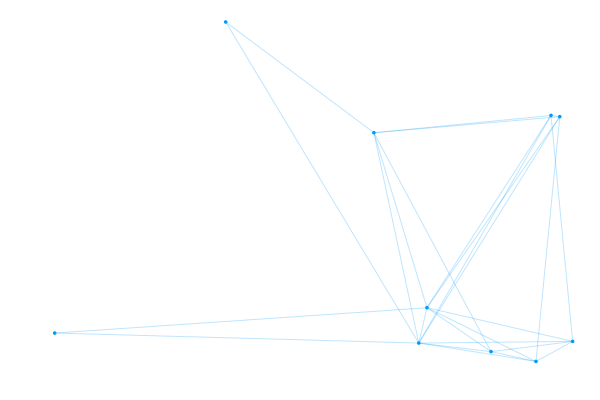
\includegraphics[width=\textwidth]{code/q5-p2.png}
	\item The starting condition $\rho$ determines the potency of spreading, as it scales the probability of being infected given the probability that a given neighbor is infected. To begin the simulation, we must first infect somebody (quite evil but anything for science). So we seal the fate of the first node by infecting it with probability 1, this is patient zero.
		\begin{lstlisting}
function evolve_steps(x0::Vector, p::Real, A::AbstractMatrix, k::Int)
	X = zeros(length(x0),k+1)
	X[:, 1] = x0
	for i=1:k
		X[:,i+1] = max.(evolve(X[:,i], p, A), X[:,1]) # fix the initial probability x0
	end
	return X
end
		\end{lstlisting}
	\item ~ \\
		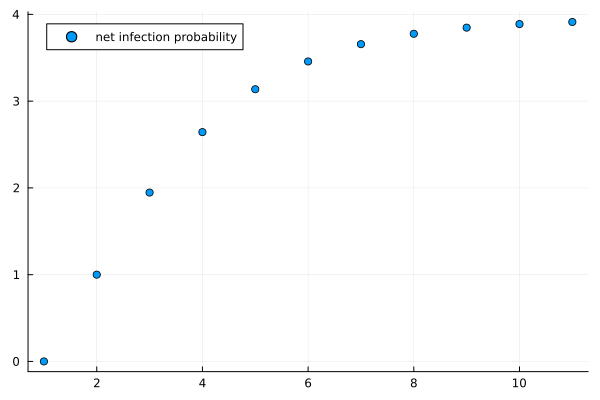
\includegraphics[width=\textwidth]{code/q5-p4.png}
		I think this plots looks looks fairly intuitive given it is monotonic. However, it seems to be approaching a steady state that doesn't leave everyone infected, so to me this is somewhat surprising. The change I would make is that instead of setting x0 as the minimum, I'd set \texttt{X[:, i]} as the minimum when computing the updated probability states, given that probability of infection for each node must remain monotonic.
	\item
		\begin{lstlisting}
function approx_evolve_steps(x0::Vector, p::Real, A::AbstractMatrix, k::Int)
	X = zeros(length(x0),k+1)
	X[:, 1] = x0
	for i=1:k
		X[:,i+1] = max.(p.*(A*X[:, i]), X[:, i])
	end
	return X
end
		\end{lstlisting}
		\begin{center}
			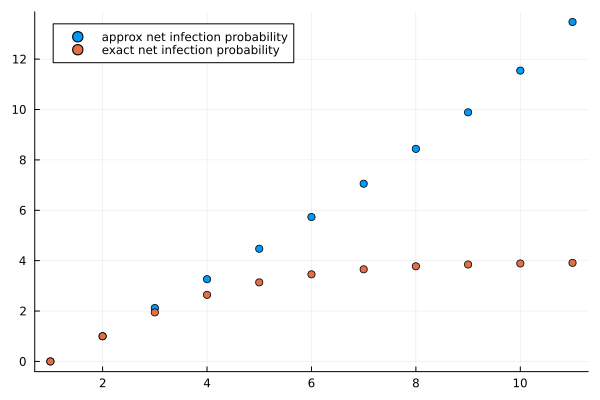
\includegraphics[width=.7\textwidth]{code/q5-p5.png}
		\end{center}
		Overlaying both, they're not very close. $\rho = .2$ is pretty aggressive so that does check out.
		I tried a couple other values, and it seems to be pretty similar as far as $\rho = .075$. \\
		\begin{center}
			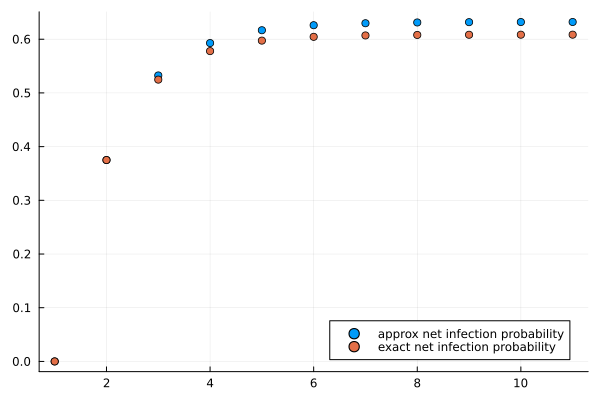
\includegraphics[width=.7\textwidth]{code/q5-p5b.png}
		\end{center}
	\item Computing exactly, we have:
		\begin{verbatim}
0.05:	2.2147609258487027
0.1:	13.284931849129581
0.15:	91.25316599696535
0.2:	187.01853110400157
		\end{verbatim}
		Computing the approximations, we have:
		\begin{verbatim}
0.05:	2.245887055423145
0.1:	17.525090005300004
0.15:	414.43051462288486
0.2:	5935.081178726405
		\end{verbatim}
	\item $f = 0.1:$
		\begin{verbatim}
Exact -
0.05:	2.1855337586969155
0.1:	10.986070393749465
0.15:	79.19958635793614
0.2:	175.4514119107722

Approximate -
0.05:	2.2158157881100586
0.1:	14.316362738700006
0.15:	298.2168370196164
0.2:	4190.310200012802
		\end{verbatim}
		$f = 0.2$
		\begin{verbatim}
Exact -
0.05:	2.069686553575516
0.1:	7.212625479439187
0.15:	48.22007277926233
0.2:	137.27831253501301

Approximate -
0.05:	2.090935256316993
0.1:	8.622585344600003
0.15:	120.20576733644496
0.2:	1594.8595357696008
		\end{verbatim}
		$f = 0.3$
		\begin{verbatim}
Exact -
0.05:	1.85344784101363
0.1:	4.73449001259144
0.15:	19.810011769879956
0.2:	76.3573538688463

Approximate -
0.05:	1.8692448553495118
0.1:	5.5370666049000015
0.15:	45.870099183829666
0.2:	539.1967444992002
		\end{verbatim}
		$f = 0.4$
		\begin{verbatim}
Exact -
0.05:	1.6508958815006438
0.1:	3.314971265463761
0.15:	9.216509725827118
0.2:	28.680290981075718

Approximate -
0.05:	1.6612361319829108
0.1:	3.6671809465000003
0.15:	16.970630170221185
0.2:	154.77591828480007
		\end{verbatim}
		$f = 0.5$
		\begin{verbatim}
Exact -
0.05:	1.6148047520808846
0.1:	2.897113115881908
0.15:	6.0135671139733216
0.2:	12.654701109935086

Approximate -
0.05:	1.6234464478638668
0.1:	3.124832097600001
0.15:	9.75216472124746
0.2:	67.11750686720002
		\end{verbatim}
		$f = 0.6$
		\begin{verbatim}
Exact -
0.05:	1.3884126229957134
0.1:	2.119473632223249
0.15:	3.8920328951181467
0.2:	7.9593681770090745

Approximate -
0.05:	1.3916229429317384
0.1:	2.1842057561000003
0.15:	4.794743637666894
0.2:	18.154333388800005
---
		\end{verbatim}
	\item Wearing masks (correctly!) would reduce the potency of the spread, given the chance of infecting another person is reduced by the barrier induced by the mask. Thus $\rho_{\mathrm{masks}} \ll \rho_{\mathrm{orig}}$, if $\rho$ is small enough, it will take significantly longer to converge. This however also de-incentivizes social distancing. Therefore treating these two variables as independent is perhaps not a solid assumption, but assuming our approximate analytical model. After $k$ steps, $\rho_{\mathrm{masks}}^k \ll \rho_{\mathrm{orig}}^k$ even if the impact over an individual step is small, the network effect is large.

\end{enumerate}

\newpage
\question
\hfill

\begin{enumerate}[label=\arabic*.]
	\item
		\begin{lstlisting}
using DelimitedFiles, LinearAlgebra, SparseArrays, Plots


coords = readdlm("chutes-and-ladders-coords.csv",',')
data = readdlm("chutes-and-ladders-matrix.csv",',')

xc = coords[:, 1]
yc = coords[:, 2]

TI = Int.(data[:,1])
TJ = Int.(data[:,2])
TV = data[:,3]
T = sparse(TI, TJ, TV, 101, 101)
A = -T' + I  #  linear system in terms of T

y = ones(101)
y[100] = 0

x = A\y
		\end{lstlisting}
		Here's the resultant plot:
		\begin{center}
			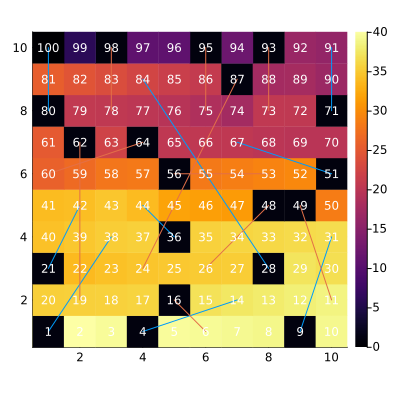
\includegraphics[width=.5\textwidth]{code/q6.png}
		\end{center}
		$x_{\{101\}} \approx 39.598$, whereas $x_{\{2\}} \approx 40.071$, which means that the start is actually \textit{not} the state with the maximum expected length. This makes intuitive sense, because we observe that the ladder on state 1 gives a significant boost to a player, sending them straight to state 38. This ladder cannot be accessed by a player on state 2.
	\item Once we are past the maximum expected number of moves for a given state, the series reduces monotonically, thus we have a lower bound of the infinite series by computing the partial sum. Once summands reduce below a given threshold (arbitrarily set as $10^{-6}$), we can stop the count.
		\begin{lstlisting}
expected_length = 0.0
delta = 1.
flag = true
k = 3
while delta > 1e-6 || flag
	global delta = k * (T^(k-1)*T[:, 101])[100]
	global expected_length += delta
	global k += 1

	if delta > 1e-6
		global flag = false # trip flag
	end
end
		\end{lstlisting}
		This program computes upto $k = 429$ and gets an expected length of $\approx 39.598$, matching our analytical solution.
\end{enumerate}

\newpage
\question
\hfill

\begin{enumerate}[label=\arabic*.]
	\item We have:
		$$
		\mU = \bmat{u(x_0, y_0) & \cdots & u(x_0, y_n) \\ \vdots & \ddots & \vdots \\ u(x_n, y_0) & \cdots & u(x_n, y_n)}
		$$
		Flattened in row-major order to $\vu$; thus $\vu_{(n + 1)i + j} = \mU_{ij}$. To simplify notation, we'll permute the order and use matrix indexing (also similarly for $\vf$ as $\mF$) with the understanding that it maps following the rule above. We linearly approximate the 2D Laplacian with $\mA \vu = \vf = \Delta \vu$. We can generalize the form up to $\mB$:
		$$
		\begin{bmatrix}
			\mI_{4n \times (n + 1)^2} \\
			\mB
		\end{bmatrix} \bmat{\mU_{00} \\ \mU_{01} \\ \vdots \\ \mU_{0,n} \\ \mU_{n, 0} \\ \mU_{n, 1} \\ \vdots \\ \mU_{nn} \\ 
		\mU_{10} \\ \vdots \\ \mU_{n - 1, 0} \\
		\mU_{1, n} \\ \vdots \\ \mU_{n - 1, n} \\
		\mU_{1,1} \\ \mU_{1,2} \\ \vdots \\ \mU_{1, n-1} \\ \mU_{2, 1} \\ \vdots \\ \mU_{n-1, n-1}}
		= \frac{1}{n^2} \bmat{\mathbf{0}_{1 \times 4n} \\ \mF_{1,1} \\ \mF_{1,2} \\ \vdots \\ \mF_{1, n-1} \\ \mF_{2, 1} \\ \vdots \\ \mF_{n-1, n-1}}
		$$
		For $n=3,~\mB = \mathbf{0}_{(n+1)^2 - 4n \times (n + 1)^2}$ except for 
		$\mB_{1,2} = \mB_{1, 2n+3} = \mB_{1, 4n + 2} = \mB_{1, 4n + 4} = 
		\mB_{2,3} = \mB_{2, 3n + 3} = \mB_{2, 4n + 1} = \mB_{2, 4n + 4} =
		\mB_{3,3n + 2} = \mB_{3, n + 3} = \mB_{3, 4n + 1} = \mB_{3, 4n + 4} =
		\mB_{4,n + 2} = \mB_{4, 4n} = \mB_{4, 4n + 2} = \mB_{4, 4n + 3} = 1$, and 
		$\mB_{1, 4n + 1} = \mB_{2, 4n + 2} = \mB_{3, 4n + 3} = \mB_{4, 4n + 4} = -4$.
	\item
		\begin{lstlisting}
using LinearAlgebra, SparseArrays, Plots

function map_index(i::Integer, j::Integer, n::Integer)
	if 1 < i < n+1 && 1 < j < n+1
		return 4n + (i - 2)*(n-1) + j-1
	elseif i == 1
		return j
	elseif i == n+1
		return n + 1 + j
	elseif j == 1
		return 2(n+1) + i - 1
	elseif j == n+1
		return 2(n+1) + n - 2 + i
	end
end

function map_index_inv(k::Integer, n::Integer)
	if k <= n+1
		return 1, k
	elseif k <= 2(n+1)
		return n + 1, k - (n+1)
	elseif k < 2(n+1) + n
		return k - 2(n + 1) + 1, 1
	elseif k <= 4n
		return k - 2(n + 1) - n + 2, n + 1
	else
		return div(k-1 - 4n, n-1) + 2, (k-1 - 4n)%(n-1) + 2
	end
end

function laplacian(n::Integer, f::Function)
	A = sparse(1I, (n+1)^2, (n+1)^2)
	A[diagind(A)[4n+1:end]] .= -4

	fvec = zeros((n+1)^2)

	global row_index = 4n + 1
	for i in 2:n
		for j in 2:n
			A[row_index, map_index(i-1, j, n)] = 1
			A[row_index, map_index(i+1, j, n)] = 1
			A[row_index, map_index(i, j-1, n)] = 1
			A[row_index, map_index(i, j+1, n)] = 1
			fvec[row_index] = f(i, j)

			global row_index += 1
		end
	end

	return A, fvec/n^2
end

n = 10
A, fv = laplacian(n, (x, y) -> 1)
		\end{lstlisting}
	\item ~
		\begin{lstlisting}
u = A\fv

U = spzeros(n+1, n+1)
for k in 4n+1:(n+1)^2
	i, j = map_index_inv(k, n)
	U[i, j] = u[k]
end

surface(U)
		\end{lstlisting}
		\begin{center}
			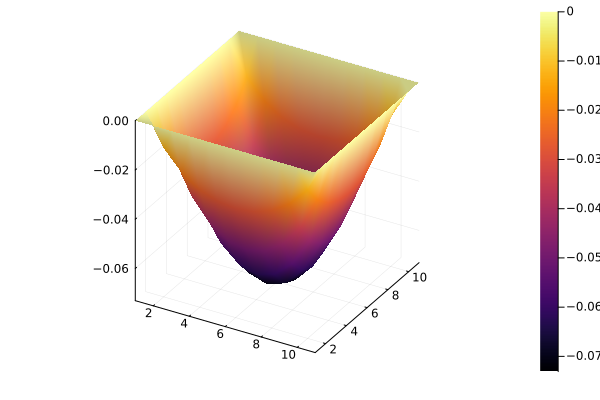
\includegraphics[width=.5\textwidth]{code/q7.png}
		\end{center}
	\item On trimming out the boundary conditions, we get a new solution $\mU'$. $\|\mU - \mU' \|_F \approx 1.96 \cdot 10^{-16}$. Thus we can exclude the boundary condition and get the same solution.
		\begin{lstlisting}
A_smol = A[4n+1:end,4n+1:end]
fv_smol = fv[4n+1:end]
u_smol = A_smol\fv_smol

norm(u_smol - u[4n+1:end])
		\end{lstlisting}
\end{enumerate}

\newpage
\question
\hfill

\begin{enumerate}[label=\arabic*.]
	\item
		\begin{lstlisting}
function csc_transpose_matvec(colptr, rowval, nzval, m, n, x)
	res = zeros(n)

	for col_idx in 1:n
		for col_ptr in colptr[col_idx]:(colptr[col_idx+1]-1)
			res[col_idx] += x[rowval[col_ptr]] * nzval[col_ptr]
		end
	end

	return res
end
		\end{lstlisting}
	\item ~
		\begin{lstlisting}
function csc_column_projection(colptr, rowval, nzval, m, n, i, x)
	res = 0
	for col_ptr in colptr[i]:(colptr[i+1]-1)
		res += x[rowval[col_ptr]] * nzval[col_ptr]
	end

	return res
end
		\end{lstlisting}
	\item ~
		\begin{lstlisting}
function csc_col_col_prod(colptr, rowval, nzval, m, n, i, j)
	res = 0
	for col_ptr_i in colptr[i]:(colptr[i+1]-1)
		for col_ptr_j in colptr[j]:(colptr[j+1]-1)
			if rowval[col_ptr_i] == rowval[col_ptr_j]
				res += nzval[col_ptr_i] * nzval[col_ptr_j]
			end
		end
	end

	return res
end
		\end{lstlisting}
	\item ~
		\begin{lstlisting}
function csc_lookup(colptr, rowval, nzval, m, n, i, j)
	for col_ptr in colptr[j]:(colptr[j+1]-1)
		if rowval[col_ptr] == i
			return nzval[col_ptr]
		end
	end

	return 0
end
		\end{lstlisting}
	\item ~
		\begin{lstlisting}
function csc_lookup_row(colptr, rowval, nzval, m, n, i)
	res = zeros(n)
	for col_idx in 1:n
		for col_ptr in colptr[col_idx]:(colptr[col_idx+1]-1)
			if rowval[col_ptr] == i
				res[col_idx] = nzval[col_ptr]
			end
		end
	end

	return res
end
		\end{lstlisting}
\end{enumerate}

\end{questions}
\end{document}
